% Capitolo 4

\chapter{Conclusioni e sviluppi futuri}
\label{Capitolo5}
\lhead{Capitolo 5. \emph{Conclusioni e sviluppi futuri}}

L'architettura e il prototipo sviluppato saranno implementati su scala
ridotta, a partire dalle comunità più strutturate e che fungono già da
poli regionali, chiamati \emph{Nucleos de Formação Continuada, (NFC)},
nuclei di formazione continua, che sono attualmente dieci,
geograficamente ben distribuiti sul territorio nazionale brasiliano.

Il codice prodotto consente una prima implementazione per un progetto
pilota che coinvolga sviluppatori del NPDD e consenta la formazione di
tecnici locali nei NFC, oltre ad ottenere un feedback diretto sull'uso
da parte delle comunità.

Attualmente il codice supporta:
\begin{itemize}
\item autenticazione LDAP (con gestione basica dei gruppi)
\item creazione e upload di contenuti audio, immagini e video
\item distribuzione tramite \emph{git-annex}
\item sincronizzazione degli oggetti sui portali django (ricreando gli
  oggetti relativi ai contenuti distribuiti via \emph{git-annex})
\end{itemize}

Da implementare e migliorare nelle prossime versioni:
\begin{itemize}
\item trasferimento selettivo dei contenuti/valori basato sull'uso
  statistico o su richiesta
\item sviluppo di in interfaccia di visualizzazione e pubblicazione
  per l'utente finale
\item gestione del DIT dell'LDAP tramite script e/o portale
\end{itemize}

% \begin{figure}[htbp]
%   \centering
%   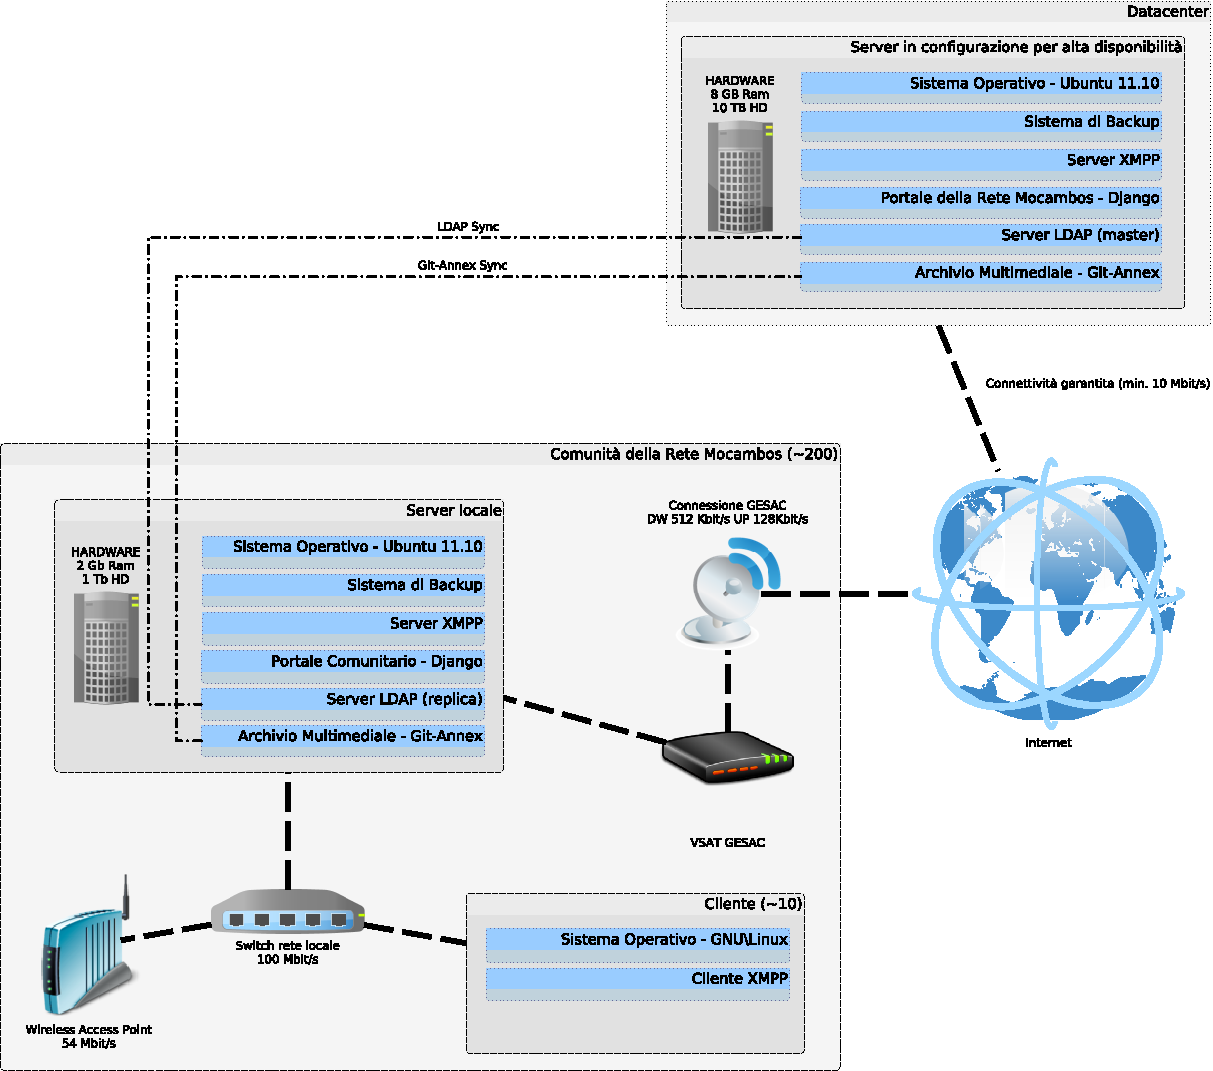
\includegraphics[width=\textwidth]{./Figure/SchemaServer_ReteMocambos-crop.pdf}
%   \rule{35em}{0.5pt}
%   \caption[Schema dell'infrastruttura della RM]{Schema dell'infrastruttura della RM.}
%   \label{fig:SchemaServer_ReteMocambos}
% \end{figure}
